\chapter{Η συνεισφορά μας}

Στο κεφάλαιο αυτό αναλύεται η δική μας συνεισφορά και τα πειράματα μας. Αρχικά, περιγράφονται αναλυτικά τo διαλογικό σύστημα \en{Rasa}, καθώς και το σύστημα ενισχυτικής μάθησης \en{Vowpal Wabbit}. Έπειτα, περιγράφεται η διαδικασία που ακολουθήσαμε, καθώς και τα προβλήματα που ανέκυψαν κατά την διαδικασία. Τέλος περιγράφεται η πλήρης αρχιτεκτονική του συστήματος και η λειτουργία του.

\section{Το διαλογικό σύστημα \en{Rasa}}

Το \en{Rasa} είναι ένα πλαίσιο (\en{framework}) ανοιχτού κώδικα για την ανάπτυξη και την έκδοση εφαρμογών συνομιλίας τεχνητής νοημοσύνης. Παρέχει ένα σύνολο εργαλείων και βιβλιοθηκών που επιτρέπουν στους προγραμματιστές να δημιουργούν διαλογικούς πράκτορες, εικονικούς βοηθούς και άλλους συνομιλητές. Το \en{Rasa} έχει σχεδιαστεί για να προσφέρει ευελιξία και έλεγχο της συμπεριφοράς και των δυνατοτήτων αυτών των συστημάτων τεχνητής νοημοσύνης.

Το πλαίσιο \en{Rasa} μπορεί νοητικά να χωριστεί σε δύο κομματια. Τα κομμάτια αυτά στο παρελθόν ήταν και ξεχωριστές υπηρεσίες, αλλά πλέον όλα βρίσκονται σε ένα πακέτο: το \en{Rasa NLU (Natural Language Understanding)} υπεύθυνο για την κατανόηση φυσικής γλώσσας και το \en{Rasa Core}.

To \en{Rasa NLU} είναι υπεύθυνο για την κατανόηση των εισροών των χρηστών και την εξαγωγή σχετικών πληροφοριών από αυτές. Χρησιμοποιεί τεχνικές μηχανικής μάθησης για την επεξεργασία και την ταξινόμηση των μηνυμάτων των χρηστών, εξάγοντας οντότητες και προθέσεις.

Το \en{Rasa Core} χειρίζεται τη διαχείριση του διαλόγου και τη διαδικασία λήψης αποφάσεων. Χρησιμοποιεί ενισχυτική μάθηση για να εκπαιδεύσει μοντέλα που μπορούν να προβλέψουν την επόμενη καλύτερη ενέργεια με βάση την τρέχουσα κατάσταση της συνομιλίας. Το \en{Rasa Core} επιτρέπει στους προγραμματιστές να ορίζουν τις ροές συνομιλιών, να χειρίζονται τις απαντήσεις των χρηστών και να διαχειρίζονται το περιβάλλον και την κατάσταση.

Ένα από τα βασικά πλεονεκτήματα του \en{Rasa} είναι η ευελιξία και η δυνατότητα προσαρμογής του. Οι προγραμματιστές μπορούν να ορίσουν τα δικά τους μοντέλα γλώσσας για συγκεκριμένο τομέα, να τους εκπαιδεύσουν χρησιμοποιώντας τα δικά τους δεδομένα και να τα βελτιστοποιήσουν για να επιτύχουν καλύτερη απόδοση. Το \en{Rasa} υποστηρίζει επίσης την ενοποίηση με άλλες υπηρεσίες και πλατφόρμες, επιτρέποντας στους προγραμματιστές να συνδέουν τους διαλογικούς τους πράκτορες τους με διάφορα κανάλια, όπως ιστότοπους, εφαρμογές ανταλλαγής μηνυμάτων και φωνητικές διεπαφές.

To \en{Rasa} βασίζεται στην ιδέα της ανάπτυξης βασισμένης στις συνομιλίες (\en{Conversation Driver Development}). Αυτό σημαίνει ότι η καλύτερη πηγή πληροφορίας για την βελτίωση του διαλογικού πράκτορα προέρχεται από τις πραγματικές συνομιλίες που δημιουργούνται από την επικοινωνία με χρήστες.

Αν και αρχικά το \en{Rasa} χρησιμοποιούσε σε μεγάλο βαθμό την ιδέα των προθέσεων για την δημιουργία των πρακτόρων, τον τελευταίο καιρό έχουν αρχίσει να δοκιμάζουν να χτίσουν εργαλεία, τα οποία θα επιτρέψουν στους πράκτορες να λειτουργήσουν χωρίς προθέσεις, δημιουργώντας ένα σύστημα άκρη-σε-άκρη (\en{end-to-end}), στο οποίο το σύστημα διαχείρισης του διαλόγου θα χρησιμοποιεί το κείμενο της απάντησης για να επιλέξει την επόμενη κατάσταση του διαλόγου, αντί να βασίζεται στην πρόθεση, όπως φαίνεται στο Σχήμα~\ref{fig:rasa_intentless}. Φυσικά, αυτό δεν σημαίνει ότι οι προθέσεις δεν έχουν χρήση, αλλά σε περιπτώσεις που το σύστημα δεν μπορεί με μεγάλη βεβαιότητα να προβλέψει την πρόθεση, η χρήση της πολιτικής χωρίς προθέσεις μπορεί να φέρει καλύτερα αποτελέσματα.

\begin{figure}
    \centering
    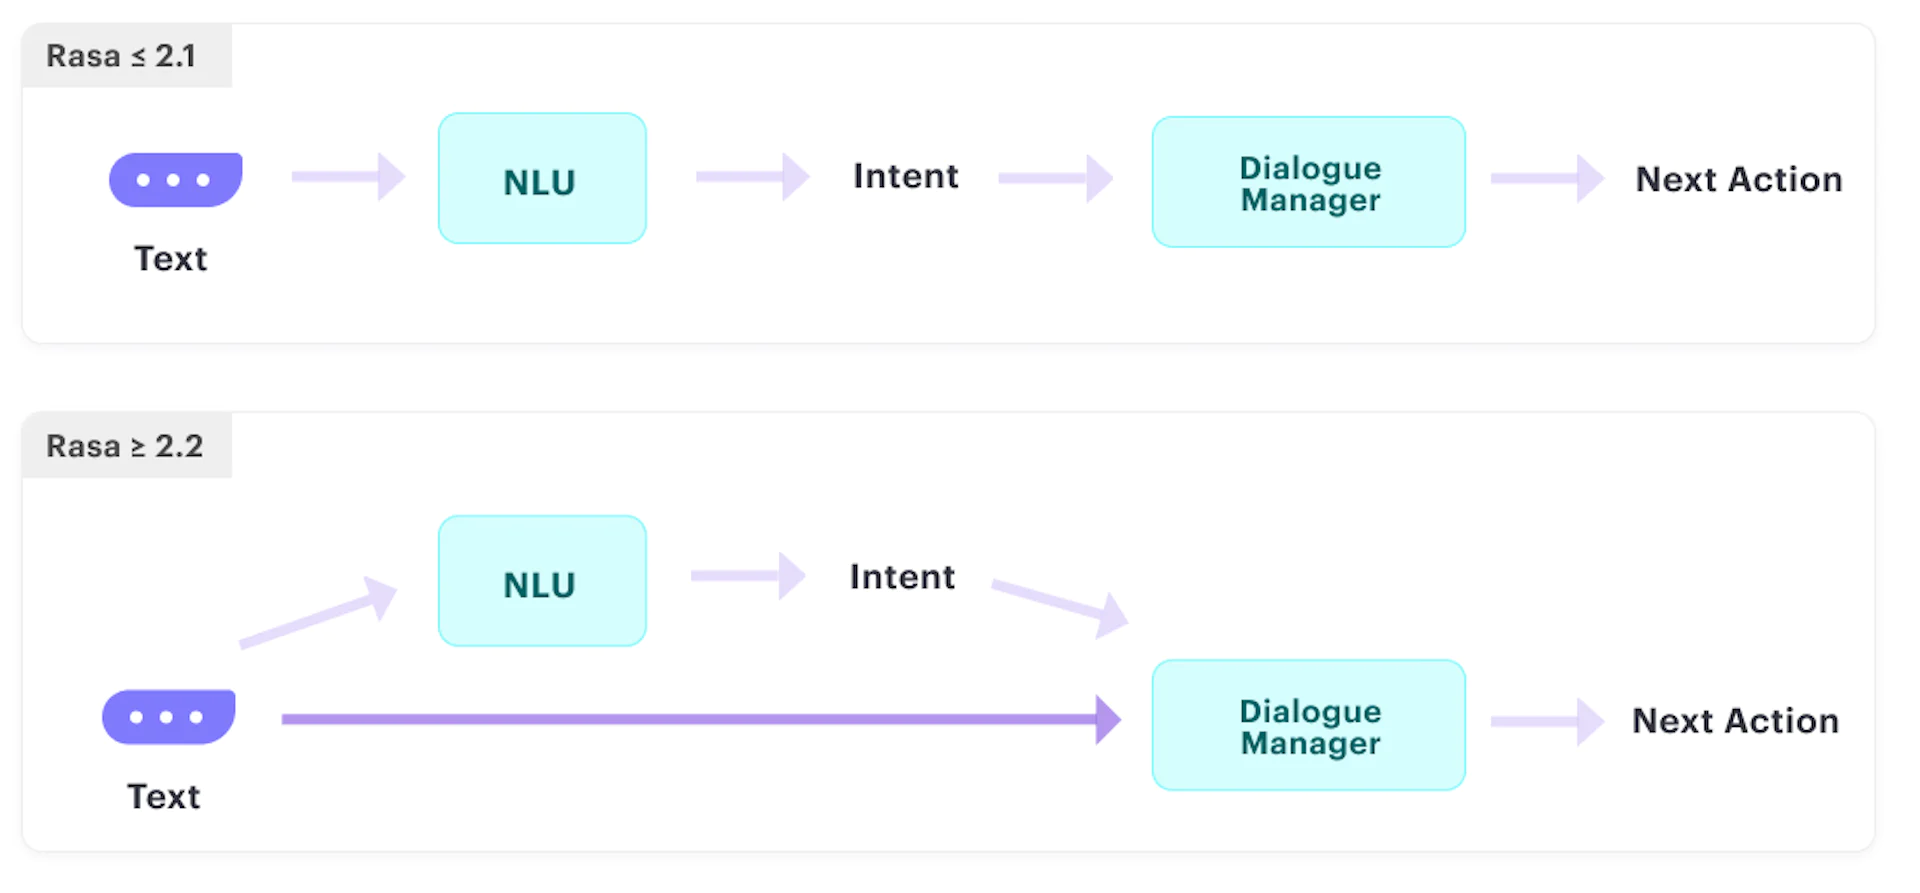
\includegraphics[width=\textwidth]{body_matter/our_work/images/rasa_intentless.png}
    \caption{Η αρχιτεκτονική του συστήματος με και χωρίς προθέσεις}
    \label{fig:rasa_intentless}
\end{figure}


\subsection{\en{Rasa NLU}}

Το \en{Rasa NLU} είναι το κομμάτι της εφαρμογής υπευθυνο για την κατανόηση της φυσικής γλώσσας. Το \en{Rasa} χρησιμοποιεί μια τεχνική η οποία ονομάζεται \en{DIET (Dual Intent and Entity Transformer)}, το οποίο είχε καλύτερα αποτελέσματα από \en{fine-tuning} ενός μοντέλου \en{BERT}, μετασχηματιστή που το 2020 θεωρούνταν τελευταίας τεχνολογίας. Το \en{DIET} έχει διττό ρόλο, καθώς διαχειρίζεται τόσο την αναγνώριση των προθέσεων, όσο και την εξαγωγή προθέσεων. H αρχιτεκτονική του \en{DIET} φαίνεται στο Σχήμα~\ref{fig:diet_architecture}.

Η δομή του μοντέλου είναι η εξής. Έστω ότι, για παράδειγμα, ο χρήστης λέει \en{"play ping pong"}, οταν ο πράκτορας τον ρωτήσει τι θα ήθελε να κάνει. Η πρόταση θα σπάσει σε λέξεις (\en{tokens}), και κάθε μια θα περάσει μέσα από ένα κομμάτι του δικτύου με δύο διαδρομές. Η πρώτη είναι η προ-εκπαιδευμένη διαδρομή, κάτα την οποία η λέξη περνάει μέσα από ένα προ-εκπαιδευμένο δίκτυο και επιστρέφει μια διανυσματική αναπαράσταση της λέξης. Αυτό το δίκτυο μπορεί να είναι κάποιος μετασχηματιστής για παράδειγμα. Η άλλη διαδρομή μετατρέπει πρώτα την λέξη σε μια αραιή αναπαράσταση της με βάση τις λέξεις και τα \en{n-grams} που δημιουργούνται και μετά περνάει μέσα από ένα νευρωνικό δίκτυο, κάνοντας την πράξη $g(Wx + b)$, όπου $x$ είναι η αραιή αναπαράσταση, $W$ τα βάρη του δικτύου και $b$ η κλίση (\en{bias}). Έπειτα τα δύο διανύσματα από τις δύο διαδρομές ενώνονται και περνάνε μέσα από ένα ακόμα νευρωνικό δίκτυο, το οποίο έχει ως έξοδο ένα διανυσμα 256 διαστάσεων. Τα νευρωνικά δίκτυα αυτά δεν είναι πλήρως συνδεδεμένα, αλλά έχουν αφαιρεθεί κάποιες ακμές με χρήση \en{drop-out}. Επιπλέον όλα τα νευρωνικά δίκτυα που βρίσκονται στο ίδιο επίπεδο, έχουν τα ίδια βάρη.

Πέρα από τις λέξεις, στο σύστημα εισέρχεται και το \en{\texttt{\_\_CLS\_\_} token}, το οποίο ουσιαστικά είναι η αναπαράσταση ολόκληρης της πρότασης. Αυτή η αναπαράσταση ουσιαστικά δημιουργείται είτε με την ένωση των διανυσμάτων των επιμέρους λέξεων, στο κομμάτι της δημιουργίας της αραιής αναπαράστασης είτε είναι η αναπαράσταση της πρότασης μέσα από το προ-εκπαιδευμένο δίκτυο.

Ακόμα, κατα την εκπαίδευση, μια από τις λέξεις συγκαλύπτεται με μια μάσκα, το \en{\texttt{\_\_MASK\_\_}}. Στο παράδειγμα του Σχήματος~\ref{fig:diet_architecture}, η λέξη αυτή είναι το \en{pong}. Αυτή η λέξη μετά θα πρέπει να προβλεφθεί από τον μετασχηματιστή. Αυτη η πρόβλεψη θα περάσει μετά από ενα δίκτυο διανυσματικής αναπαράστασης και θα συγκριθεί με την πραγματική λέξη. Αυτό μας δείχνει πόσο καλά το μοντέλο μας μπορεί να γενικεύσει την γλώσσα.

Ακόμα, κατά την εκπαίδευση, μια παρόμοια διαδικασία συμβαίνει μεταξύ του \en{\texttt{\_\_CLS\_\_} token} και της (γνωστής) πρόθεσης του χρήστη, καθώς στηριζόμαστε στην ιδέα ότι το \en{token}, αφού αναπαριστά ολόκληρη την πρόταση, φέρει πληροφορία σχετικά με την πρόθεση.

Τέλος, οι λέξεις αφού περάσουν μέσα από τον μετασχηματιστή, συγκρίνονται με τις πραγματικές οντότητες που αναπαριστούν μέσα σε ένα υπό συνθήκη τυχαίο πεδίο (\en{Conditional Random Field}) και υπολογίζεται μια απώλεια.

Έτσι το σύστημα ολόκληρο εκπαιδεύεται με βάση την συνολική απώλεια που προκύπτει από το σφάλμα στην αναγνώριση οντοτήτων, στην πρόβλεψη της λέξης μέσα στην πρόταση και την κατανοηση της πρόθεσης του χρήστη.
\begin{figure}
    \centering
    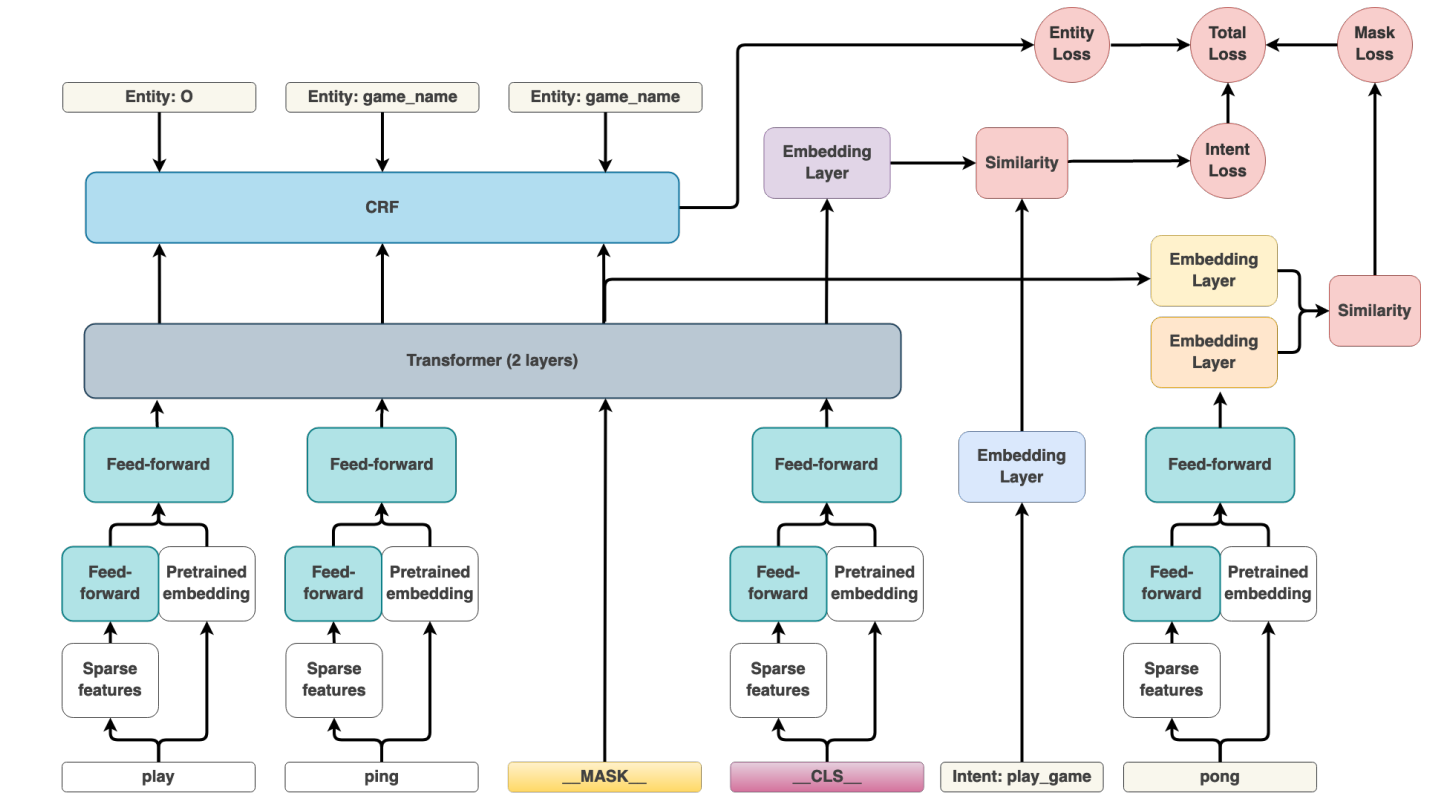
\includegraphics[width=\textwidth]{body_matter/our_work/images/DIET_architecture.png}
    \caption{Η αρχιτεκτονική του συστήματος \en{DIET}\cite{bunk2020diet}}
    \label{fig:diet_architecture}
\end{figure}

\subsection{\en{Rasa Core}}

Στο κομμάτι αυτό γίνεται η διαχείριση του διαλόγου και η επιλογή της επόμενης κίνησης. Ακόμα γίνεται η παραγωγή του διαλόγου. Θα εξηγήσουμε περιληπτικά το πώς λειτουργούν τα μέρη αυτά.

Το \en{Rasa} χρησιμοποιεί ένα σύνολο από πολιτικές για την διαχείριση του διαλόγου, και ανάλογα με την προτεραιότητα τους και την εμπιστοσύνη που έχουν στην πρόβλεψη τους, επιλέγει ποια θα χρησιμοποιήσει.

Μια από τις πιο σημαντικές είναι η πολιτική \en{TED (Transformer Embedding Dialogue)}.Η πολιτική \en{TED} χρησιμοποιείται για την επιλογή της επόμενης ενέργειας και την αναγνώριση οντοτήτων. Για την επιλογή της ενέργειας, η πολιτική ενώνει σε ένα διάνυσμα την αναπαράσταση της προηγούμενης πράξης, της πρόθεσης και πληροφοριών που είναι απαραίτητο να είναι διαθέσιμες μακροχρόνια (όπως πληροφορίες από κάποια φόρμα). Έπειτα, αυτές περνάνε μέσα από ένα μετασχηματιστή, παρέα με τις αναπαραστάσεις των προηγούμενων καταστάσεων. Η έξοδος του μετασχηματιστή περνάει μέσα από ένα νευρωνικό δίκτυο όπου γίνεται η πρόβλεψη της πρότασης που θα κάνει το σύστημα, μαζί με μια βεβαιότητα στην πρόταση αυτή.

Με αυτό τον τρόπο, το σύστημα μπορεί να διαχειριστεί την επικοινωνία με τον χρήστη όταν αυτός ξεφεύγει από το χαρούμενο μονοπάτι και μπορεί να επιστρέψει στην αρχική συζήτηση. Για την εκπαίδευση αυτού του συστήματος, χρησιμοποιούνται δεδομένα, τα οποία λέγονται ιστορίες (\en{stories}). Οι ιστορίες αυτές περιγράφουν τα διαλογικά μονοπάτια των χρηστών, και είναι η βάση της ανάπτυξης με βάση την συνομιλία. Καθώς οι χρήστες χρησιμοποιούν τον διαλογικό πράκτορα και κάνουν συζητήσεις μαζί του, οι προγραμματιστές μπορούν να αναγνωρίσουν ποια ειναι τα πιο συχνά καλά ή κακά μονοπάτια που παίρνουν και να τα καταγράψουν σαν ιστορίες για να εκπαιδευτεί ο πράκτορας να τα διαχειρίζεται.

Οσον αφορά το κομμάτι της παραγωγής διαλόγου, αυτό βασίζεται πάνω στην ιδέα των προτύπων (\en{templates}). Ο προγραμματιστής για κάθε δράση προσθέτει πρότυπα απαντήσεων μαζί με θέσεις όπου μπορούν να μπουν συγκεκριμένες πληροφορίες οι οποίες προέρχονται από τον χρήστη.

\subsection{\en{Rasa Action Server}}

Πέρα από τα παραπάνω, ένα σημαντικό κομμάτι για την εργασία μας είναι οι προσαρμοσμένες ενέργειες (\en{custom actions}), οι οποίες υλοποιούνται στον \en{Rasa Action Server}. Η υπηρεσία αυτή επιτρέπει στους προγραμματιστές να γράψουν ενέργειες οι οποίες είναι προσαρμοσμένες στο τί θέλουμε να κάνουμε. Το \en{Rasa} στέλνει στον \en{Action server} ενα αίτημα με πληροφορίες όπως την δράση που προβλέφθηκε, το αναγνωριστικό της συζήτησης, την καταγραφή ολόκληρης της συζήτησης και τα περιεχόμενα του περιβάλλοντος του πράκτορα. Με βάση αυτά, ο \en{action server} επιστρέφει απαντήσεις και γεγονότα τα οποία θα χρησιμοποιήσει μετά το \en{Rasa} για αν απαντήσει στον χρήστη.

\section{\en{Vowpal Wabbit}}

Το \en{Vowpal Wabbit}\cite{agarwal2013reliable} είναι μια βιβλιοθήκη μηχανικής μάθησης ανοιχτού κώδικα, η οποία αναπτύχθηκε αρχικά στα εργαστήρια της \en{Yahoo}, και πλέον αναπτύσσεται από την ερευνητική ομάδα της \en{Microsoft}. Το όνομα "\en{Vowpal Wabbit}" είναι παιχνιδισμός στην φράση  "\en{vorpal wabbit}" από το ποίημα του Λιούις Κάρολ "\en{Jabberwocky}".

Το \en{Vowpal Wabbit} είναι διάσημο για την αποδοτικότητα του και την επεκτασιμότητα του, αφού είναι ικανό να διαχειριστεί δεδομένα πολλών \en{terrabyte} και να εκτελέσει σύγχρονη εκπαίδευση πολύ γρήγορα. Χρησιμοποιεί έναν σύγχρονο αλγόριθμο κατάβασης κλίσης για να ανανεώσει τα μοντέλα σταδιακά, καθώς έρχονται νέα δεδομένα. Αυτό του επιτρέπει την αποδοτική επεξεργασία ροών δεδομένων ή δεδομένων με μεγάλο αριθμό παραδειγμάτων.

Επιπλέον, το \en{Vowpal Wabbit} είναι διάσημο για τα εργαλεία διαδραστικής μάθησης που προσφέρει, όπως είναι το \en{Contextual Bandits} αλλά και άλλες μορφές ενισχυτικής μάθησης. Τέλος, προσφέρει εργαλεία τόσο για σύγχρονη όσο και για ασύγχρονη εκπαίδευση των μοντέλων.

Τα κύρια χαρακτηριστικά του \en{Vowpal Wabbit} που το κάνουν ένα εξαιρετικά δυνατό εργαλείο είναι:

\begin{enumerate}
    \item \textbf{Μορφή εισαγωγής των δεδομένων}. Η μορφή εισόδου για τον αλγόριθμο εκμάθησης είναι ουσιαστικά πιο ευέλικτη από ό,τι θα περίμενε κανείς. Τα παραδείγματα μπορεί να έχουν χαρακτηριστικά που αποτελούνται από κείμενο ελεύθερης μορφής, το οποίο ερμηνεύεται με έναν τρόπο \en{bag-of-words}. Μπορεί ακόμη να υπάρχουν πολλά σύνολα κειμένου ελεύθερης μορφής σε διαφορετικούς χώρους ονομάτων.
    \item \textbf{Ταχύτητα} Ο αλγόριθμος εκμάθησης είναι αρκετά γρήγορος --- παρόμοιος με τις λίγες άλλες βιβλιοθήκες σύγχρονων αλγορίθμων μάθησης εκεί έξω. Για παράδειγμα, μπορεί να εφαρμοστεί αποτελεσματικά σε μαθησιακά προβλήματα με αραιά σύνολα δεδομένων μεγέθους \en{terrabyte} (για παράδειγμα 1012 αραιά χαρακτηριστικά). Ως άλλο παράδειγμα, είναι περίπου 3 φορές πιο γρήγορο από το \en{svmsgd} του \en{Leon Bottou} στο παράδειγμα \en{RCV1} στο συνολικό χρόνο εκτέλεσης.
    \item \textbf{Επεκτασιμότητα} Η επεκτασιμότητα είναι διαφορετική από την ταχύτητα. Το σημαντικό χαρακτηριστικό εδώ είναι ότι το αποτύπωμα μνήμης του προγράμματος είναι ανεξάρτητο από το πλήθος των δεδομένων. Αυτό σημαίνει ότι το σετ εκπαίδευσης δεν φορτώνεται στην κύρια μνήμη πριν ξεκινήσει η εκπαίδευση. Επιπλέον, το μέγεθος του συνόλου των χαρακτηριστικών περιορίζεται ανεξάρτητα από τον όγκο των δεδομένων εκπαίδευσης χρησιμοποιώντας τεχνικές κατακερματισμού.
    \item \textbf{Σύζευξη χαρακτηριστικών (\en{feature pairing})} Τα υποσύνολα χαρακτηριστικών μπορούν να αντιστοιχιστούν εσωτερικά έτσι ώστε ο αλγόριθμος να είναι γραμμικός στο εξωτερικό γινόμενο των υποσυνόλων. Αυτό είναι χρήσιμο για προβλήματα κατάταξης. Ο \en{David Grangier} φαίνεται να έχει ένα παρόμοιο κόλπο στον κώδικα \en{PAMIR}. Η εναλλακτική λύση της ρητής επέκτασης των χαρακτηριστικών πριν από την τροφοδοσία τους στον αλγόριθμο εκπαίδευσης μπορεί να είναι τόσο εντατική σε υπολογισμούς όσο και σε χώρο, ανάλογα με τον τρόπο χειρισμού της.
\end{enumerate}

\section{Προϋπάρχουσα αρχιτεκτονική - Θεανώ}

Το σύστημα πάνω στο οποίο η εργασία βασίστηκε ονομάζεται Θεανώ. H Θεανώ είναι η διαλογική βοηθός του Ερευνητικού Κέντρου “Αθηνά”, με σκοπό να δώσει έγκυρες πληροφορίες για τον κορωνοϊό. Η υλοποίηση έγινε από τους ερευνητές του Ινστιτούτου Επεξεργασίας του Λόγου.

Η Θεανώ έχει στόχο να κρατάει ενήμερους τους πολίτες για την εξέλιξη της πανδημίας, ώστε να μπορούν να παίρνουν αποφάσεις με βάση τις οδηγίες των ειδικών, καθώς και να μειώνει τον πανικό, προσφέροντας τη δυνατότητα αυτοαξιολόγησης των συμπτωμάτων.

Παρέχει πληροφορίες για τα νέα κρούσματα και τους θανάτους στην Ελλάδα, σε χώρες του εξωτερικού και συνολικά στον κόσμο. Γνωρίζει για την πληρότητα σε ΜΕΘ και για τον αριθμό των ατόμων που έχουν εμβολιαστεί σε μια συγκεκριμένη ημερομηνία ή συνολικά στην Ελλάδα. Καλύπτει πληθώρα συχνών ερωτήσεων, όπως από που ξεκίνησε ο κορωνοϊός, πώς μεταδίδεται, ποια είναι η σωστή χρήση της μάσκας κ.λπ.

Επιπλέον, η Θεανώ βρίσκει φαρμακεία σχεδόν σε όλες τις πόλεις-περιοχές της Ελλάδας, ενώ με 6 απλές ερωτήσεις, σαν ένα μικρό διαγνωστικό τεστ, βοηθά τους χρήστες που έχουν συμπτώματα να αναγνωρίσουν αν υπάρχει πιθανότητα να είναι φορείς ή όχι.

H Θεανώ είναι χτισμένη πάνω στο \en{Rasa}. Συγκεκριμένα, χρησιμοποιεί το \en{DIET} για την αναγνώριση προθέσεων, και την πολιτική \en{TED} για την διαχείριση του διαλόγου. Επιπλέον, χρησιμοποιεί το \en{Duckling}, γραμμένο από την \en{Facebook} για την εξαγωγή οντοτήτων. Ακόμα,για να να μπορέσει η Θεανώ να διαχειριστεί τα \en{greeklish}, στην αρχή της επεξεργασίας της πρότασης του χρήστη, χρησιμοποιεί ένα μεταφραστή από \en{greeklish} σε Ελληνικά, γραμμένο στο Αθηνά.


Όσον αφορά τις δράσεις, για κάθε πρόθεση του χρήστη, υπάρχει η αντίστοιχη λειτουργικότητα στον \en{Action Server}. Ακόμα, λόγω του γεγονότος ότι η Θεανώ λειτουργούσε κάποιο καιρό πριν την εργασία μας, υπάρχουν ήδη ιστορίες που διαχειρίζονται τις περισσότερες καταστάσεις.

Όσον αφορά το κομμάτι που εργαστήκαμε εμείς, πριν την έναρξη της εργασίας, υπήρχε ήδη μια δράση, η οποία εμφανιζόταν μετά από τις απαντήσεις της Θεανώς η οποία καλούνταν με κάποια μη-μηδενική πιθανότητα και τυχαία πρότεινε κάποια από τις υπόλοιπες λειτουργίες της που δεν είχαν συζητηθεί με τον χρήστη ακόμα. Ο στόχος ήταν η διατήρηση του ενδιαφέροντος του χρήστη για μεγαλύτερο χρονικό διάστημα δίνοντας του περισσότερα θέματα για συζήτηση.

\section{Στόχοι, περιορισμοί και παραδοχές}

Στόχος της εργασίας ήταν η δημιουργία και ενσωμάτωση ενός συστήματος ενισχυτικής μάθησης στην Θεανώ.Το σύστημα αυτό θα βοηθήσει την Θεανώ να κάνει συστάσεις στον χρήστη σχετικά με θέματα που είναι σχετικά με τα ως τώρα ενδιαφέροντα του και την συνομιλία που έχει κάνει με την Θεανώ. Κάποιοι βασικοί περιορισμοί που προέρχονται από την εως τώρα λειτουργία του συστήματος μας και οι τρόποι που μας επηρεάζουν είναι οι παρακάτω:

\begin{itemize}
    \item \textbf{Περιορισμένες πληροφορίες χρηστών}: Καθώς το σύστημα δεν κρατάει κάποιο ιστορικό συνομιλιών, και δεν έχει προηγούμενη γνώση των χρηστών που αλληλεπιδρούν με αυτό, οι πληροφορίες που έχουμε για αυτούς προέρχονται μόνο μέσα από τις ερωτήσεις που κάνουν οι ίδιοι κατά την διάρκεια των συνομιλιών. Αυτό σημαίνει πώς σε κάθε συνομιλία, ο πράκτορας ξεκινάει με μηδενική γνώση του συνομιλητή και θα πρέπει μέσα από τις περιορισμένες συναναστροφές του να εξάγει πληροφορίες σχετικά με τα θέματα που μπορεί να είναι ενδιαφέροντα σε αυτόν.
    \item \textbf{Περιορισμένα ιστορικά δεδομένα}: Για να μπορέσει το σύστημα να κάνει προτάσεις, θα πρέπει να έχει εκπαιδευτεί στο τί οι χρήστες συσχετίζουν κατα την διάρκεια μιας συνομιλίας. Για να το κάνουμε αυτό εκπαιδεύσαμε το μοντέλο βασιζόμενοι στην τυχαία πολιτική την οποία είχε εως τώρα η Θεανώ. Η τεχνική αυτή ασύγχρονης εκπαίδευσης έχει τον περιορισμό ότι βασίζεται σε περιορισμένα δεδομένα. Τα ιστορικά δεδομένα στην κατοχή μας από την χρήση της Θεανώς είναι $468$ συνομιλίες, με συνολικά $1043$ τυχαίες συστάσεις, τις οποίες μπορούμε να χρησιμοποιήσουμε.
\end{itemize}

Με βάση τα παραπάνω, πήραμε τις επόμενες σχεδιαστικές αποφάσεις:

\begin{itemize}
    \item Αν θεωρήσουμε κάθε συνομιλία ως μοναδική και προσπαθήσουμε να λύσουμε το πλήρες πρόβλημα της ενισχυτικής μάθησης, θα είχαμε μόλις $468$ δείγματα, από τα οποία μόλις $261$ περιέχουν οποιαδήποτε σύσταση από την Θεανώ. Για να αυξήσουμε την ποσότητα των δεδομένων που έχουμε, καθώς και για να απλοποιήσουμε το πρόβλημα, κάνουμε την παραδοχή ότι η σειρά που γίνονται οι προτάσεις, καθώς και τα ερωτήματα του χρήστη σχετικά με πληροφορίες δεν επηρεάζουν το τι θα ενδιαφέρει τον χρήστη. Έτσι κάθε πρόταση μπορεί να γίνει μόνο με βάση τα θέματα που γνωρίζει η Θεανώ ότι έχουν συζητηθεί και ανεξάρτητα από την σειρά που συζητήθηκαν. Έτσι μπορούμε πρακτικά να αντιμετωπίσουμε το πρόβλημα σαν ένα πρόβλημα \en{contextual bandits}.
    \item Η προσαρμοσμένη ενέργεια  του \en{Action Server}, η οποία είναι υπεύθυνη για την πρόταση επόμενου θέματος καλείται σε συγκεκριμένες περιπτώσεις και όχι μετά από κάθε απάντηση του χρήστη. Αυτό κάνει δύσκολη την εύρεση της ανταμοιβής μέσα στο ιστορικό της συνομιλίας. Οπότε ένα πρόβλημα που έπρεπε να λύσουμε είναι το πώς θα γίνει η καταγραφή της ανταμοιβής με τρόπο εύρωστο, ώστε να μπορεί να καταγράφεται ανεξάρτητα της απάντησης και της αντίδρασης του χρήστη.
\end{itemize}

\section{Ανάλυση δεδομένων \& αναπαράσταση τους}

Το πρώτο βήμα για την δημιουργία του μοντέλου μας ήταν η κατανόηση των ιστορικών δεδομένων στην κατοχή μας και μετέπειτα η εκπαίδευση του μοντέλου με βάση αυτό.

Τα ιστορικά δεδομένα που έχουμε στην κατοχή μας προέρχονται από την αλληλεπίδραση της Θεανώς με το ευρύ κοινό την περίοδο 4 Οκτωβρίου 2021 μέχρι 11 Ιανουαρίου 2022. Τα δεδομένα αυτά είναι σε μορφή \en{JSON}, όπως προέρχονται από την καταγραφή του διαλόγου του \en{Rasa}. Από αυτές τις συζητήσεις, $151$ δεν έχουν κανένα γύρο μεταξύ χρήστη και της Θεανώς. Κάποια στατιστικά από τα δεδομένα φαίνονται στο Πίνακα~\ref{tab:historic_data}.

\begin{table}
    \centering
    \begin{tabular}{|c|c|}
        \hline
        Συνολικές συνομιλίες                & $468$     \\
        \hline
        Κενές συνομιλίες                    & $151$     \\
        \hline
        Συνομιλίες με σύσταση               & $261$     \\
        \hline
        Συνολικές συστάσεις                 & $1043$    \\
        \hline
        Μέσο πλήθος μηνυμάτων χρήστη        & $5.68$    \\
        \hline
        Μέσο πλήθος μηνυμάτων Θεανώς        & $9.25$    \\
        \hline
        Μέσο πλήθος συστάσεων ανα συνομιλία & $2.23$    \\
        \hline
        Επιτυχία τυχαίας πολιτικής          & $45.93\%$ \\
        \hline
    \end{tabular}
    \caption{Στατιστικά από την ανάλυση των ιστορικών δεδομένων}
    \label{tab:historic_data}
\end{table}

Όπως φαίνεται, από τα αρχικά δεδομένα θα πρέπει να γίνει κάποιος διαχωρισμός ώστε να διατηρηθούν μόνο αυτά που είναι πράγματι χρήσιμα σε εμας, δηλαδή οι $1043$ συστάσεις. Για να φτιάξουμε τα δεδομένα σε μορφή που να είναι κατάλληλη για το \en{Vowpal Wabbit}, θα πρέπει να εξάγουμε πληροφορίες για την κάθε σύσταση. Για αυτές συλλέξαμε τις προηγούμενες προθέσεις του χρήστη και τις προηγούμενες συστάσεις της Θεανώς και τις ενώσαμε για να δημιουργήσουμε το συγκείμενο (\en{context}) για κάθε σύσταση.

Οι πληροφορίες που περιέχει το συγκείμενο παίζουν αρκετά μεγάλο ρόλο στις συστάσεις στην περίπτωση μας, καθώς το συγκείμενο περιγράφει ουσιαστικά τα χαρακτηριστικά που λαμβάνει υπόψιν του το \en{Vowpal Wabbit} για να επιλέξει την σύσταση. Μια επιλογή που δοκιμάσαμε ήταν η ύπαρξη ως συγκείμενο μόνο των θεμάτων που μπορεί να προτείνει σαν σύσταση η Θεανώ. Αυτή όμως η προσέγγιση δημιουργεί ένα πολύ περιορισμένο συγκείμενο, και πολλές φορές δεν υπήρχε συγκείμενο στα παραδείγματα, ειδικά στην αρχή του διαλόγου. Μια άλλη προσέγγιση θα ήταν η χρήση όλων των προθέσεων σαν συγκείμενο. Αυτό όμως δημιουργεί ένα πολύ πιο σύνθετο συγκείμενο, για το οποίο τελικά υπάρχουν πολύ λίγα παραδείγματα, ενώ αρκετές προθέσεις δεν έχουν πραγματική αξία, όταν σκεφτόμαστε τον διάλογο (πχ η πρόθεση "\en{affirmative}"). Οπότε τελικά καταλήξαμε σε ένα συμβιβασμό μεταξύ των δύο αυτών προσεγγίσεων, κατά τον οποίο επιλέξαμε ένα υποσύνολο των προθέσεων, τα οποία δεν θεωρούμε σημαντικά και δεν έχουμε λόγο να χρησιμοποιήσουμε ως συγκείμενο, ενώ όλες οι υπόλοιπες προθέσεις προστιθενται σε αυτό.

Για να δημιουργηθεί το συγκείμενο, αφαιρούμε κάποιες από τις προθέσεις του χρήστη οι οποίες δεν προσφέρουν πληροφορία για τα ενδιαφέροντα του. Κάποιες από αυτές τις προθέσεις που αφαιρούνται είναι η θετική και η αρνητική απάντηση, οι ερωτήσεις που είναι ουσιαστικά ψιλοκουβέντα (\en{chit-chat}) - ερωτήσεις όπως τί είναι το Αθηνά, ποιο είναι το όνομα σου κλπ -, καθώς και ερωτήσεις που έχουν σχέση με την συμπλήρωση κάποιας μακροχρόνιας πληροφορίας. Αυτό θεωρήσαμε ότι θα μας βοηθήσει, καθώς το συγκείμενο είναι αρκετά μικρότερο έτσι και μας επιτρέπει να εστιάσουμε μόνο στις πράξεις που έχουν αξία για τον χρήστη.

Επιπλέον, για κάθε σύσταση θα πρέπει να βρούμε την ανταμοιβή και να την προσδιορίσουμε αριθμητικά. Για την περίπτωση μας, επιλέξαμε μια δυαδική αξιολόγηση. Ο τρόπος που προσδιορίσαμε αν μια σύσταση ήταν επιτυχημένη ή όχι ήταν ο εξής. Θεωρούμε ότι η απάντηση του χρήστη είναι αρνητική, αν:
\begin{itemize}
    \item Ο χρήστης κλείσει την συνομιλία, αρα δεν υπάρχουν περαιτέρω απαντήσεις του χρήστη.
    \item Δεν υπάρχει απάντηση από τον χρήστη για κάποιο λόγο.
    \item Αν η απάντηση του χρήστη στην σύσταση είναι αρνητική ή δεν είναι σχετική.
    \item Αν ο χρήστης ζητήσει να συζητηθεί κάποιο άλλο θέμα.
\end{itemize}
Στις υπόλοιπες περιπτώσεις θεωρούμε ότι η απάντηση του χρήστη ήταν θετική. Ενδεικτικά, τα δεδομένα από μια συζήτηση μπορούν να βρεθούν στον Πίνακα~\ref{tab:sample_conversation}. To "\en{no\_action}" ουσιαστικά υποδηλώνει την γενική ερώτηση "Θα ήθελες να μάθεις για κάποιο άλλο θέμα?".

\begin{table}
    \centering
    \begin{tabularx}{\textwidth}{|p{0.7cm}|X|X|X|X|X|}
        \hline
        A/A & Προηγούμενες προθέσεις χρήστη                                                    & Προηγούμενες συστάσεις & Συγκείμενο                  & Τρέχουσα σύσταση & Αποτέλεσμα \\
        \hline
        1   & \en{affirmative, covid\_stats}                                                   &                        & \en{covid\_stats}           & \en{no\_action}  & ΔΕΚΤΗ      \\
        \hline
        2   & \en{affirmative, covid\_stats, vaccines}                                         & \en{no\_action}        & \en{covid\_stats, vaccines} & \en{no\_action}  & ΔΕΚΤΗ      \\
        \hline
        3   & \en{affirmative, covid\_stats, vaccines, covid\_stats, greetings, ask\_chitchat} & \en{no\_action}        & \en{covid\_stats, vaccines} & \en{no\_action}  & MH ΔΕΚΤΗ   \\
        \hline
    \end{tabularx}
    \caption{Παράδειγμα συζήτησης}
    \label{tab:sample_conversation}
\end{table}

\section{Εκπαίδευση του μοντέλου}

Για την εκπαίδευση του μοντέλου χρησιμοποιήσαμε την ασύγχρονη αξιολόγηση πολιτικής \en{offline policy evaluation (OPE)} του \en{Vowpal Wabbit}.

Στόχος της τεχνικής αυτής, σε ένα περιβάλλον \en{contextual bandits} είναι η χρήση δεδομένων, τα οποία έχουν δημιουργηθεί από μια άλλη πολιτική (ας την ονομάσουμε την πολιτική που χρησιμοποιείται στην παραγωγή, στην περίπτωση μας είναι η τυχαία πολιτική) με στόχο την εκτίμηση την αξίας μιας νέας υποψήφιας πολιτικής ασύγχρονα, χωρίς την χρήση της στην παραγωγή. Η χρησιμότητα είναι ότι έτσι μπορούμε να εκτιμήσουμε την απόδοση μιας πολιτικής, χωρίς να την εκθέσουμε στο περιβάλλον παραγωγής, και να την συγκρίνουμε με την υπάρχουσα.

Όσον αφορά την αναπαράσταση των δεδομένων, το \en{Vowpal Wabbit}, έχει το δικό του τρόπο να τα αναπαριστά τα παραδείγματα καταστάσεων. Συγκεκριμένα ο τρόπος αυτός είναι ο παρακάτω:

\begin{otherlanguage}{english}
    \begin{lstlisting}[caption=Μορφή εισόδου \en{Vowpal Wabbit}]
shared |test_types find_new_icus covid_stats
2:1.0:0.1 |ill_questionnaire_form
|vaccine_stats_form
|pharmacy_form
|ways_of_protection
|symptoms
|test_cost
|what_to_do_if_positive
|underlying_conditions
|no_action
    \end{lstlisting}
\end{otherlanguage}

οπου, με την γραμμή \en{shared} δηλώνουμε ποιο είναι το συγκείμενο για την συγκεκριμένη κατάσταση, ενώ όλες οι επόμενες γραμμές δηλώνουν τις δράσεις που μπορεί να πάρει η πολιτική. Η πρώτη γραμμή σε αυτή την περίπτωση μας δείχνει την επιλογή που έκανε η τυχαία πολιτική. Συγκεκριμένα υπάρχουν 3 πεδία πριν την δράση, τα οποία χωρίζονται με άνω κάτω τελεία. Το $2$ δηλώνει τον αριθμό της δράσης, και δεν επηρεάζει τον αλγόριθμο που χρησιμοποιούμε. Το δεύτερο πεδίο ($1.0$) δηλώνει την ανταμοιβή της δράσης που επιλέχθηκε. Αρα στο παράδειγμα, ο χρήστης αποδέχτηκε την σύσταση. Το τελευταίο πεδίο υποδηλώνει την πιθανότητα να επιλεχθεί η συγκεκριμένη δράση από την τυχαία πολιτική.  Κάθε παράδειγμα τελειώνει με μια νέα γραμμή.

\subsection{Ασύγχρονη εκπαίδευση}

Σε περιβάλλοντα επιβλεπουσης μάθησης, η κλασική προσέγγιση στην ασύγχρονη εκπαίδευση είναι η εκπαίδευση στο σύνολο δεδομένων για εκπαίδευση και η εκτίμηση της γενικευμένης απόδοσης σε ένα σύνολο αξιολόγησης. Σε περιβάλλοντα σύγχρονης εκπαίδευσης, συνήθως χρησιμοποιείται η προοδευτική επαλήθευση. Σε περιβάλλοντα \en{contextual bandits} κανένα από τα δύο δεν είναι δυνατα, καθώς όπως σε όλα τα προβλήματα ενισχυτικής μάθησης, το πρόβλημα είναι ένα προβλημα μερικών πληροφοριών: δεν μαθαίνουμε ποτέ τις ανταμοιβές για τις επιλογές που δεν έγιναν. Η μόνη πηγή πληροφορίας είναι τα δεδομένα	που δημιουργούνται από την πολιτική στην παραγωγή, που μπορεί να κάνει πολύ διαφορετικές επιλογές από την υποψήφια πολιτική.

Για να γίνει εκτίμηση πολιτικών \en{contextual bandits} ασύγχρονα, είναι η χρήση εκτιμητών, οι οποίοι δημιουργούν ψεύτικες ανταμοιβές για τις πράξεις που δεν επιλέχθηκαν, δημιουργώντας έτσι ένα 'ψεύτικο' σύνολο δεδομένων επιβλέπουσας μάθησης, με βάση το οποίο μπορεί να εκτιμηθεί η απόδοση, χρησιμοποιώντας είτε προοδευτική επαλήθευση ή ένα σύνολο αξιολόγησης.

Το  \en{Vowpal Wabbit} έχει υλοποιημένους αρκετούς εκτιμητές για να μετατρέψει την αξιολόγηση πολιτικής σε αξιολόγηση επιβλεπόμενης μάθησης. Η πιο απλή μέθοδος, είναι η απευθείας μέθοδος (\en{direct method}), η οποία εκπαιδεύσει ένα μοντέλο παλινδρόμησης το οποίο εκτιμάει το κόστος (αρνητική ανταμοιβή) ενός ζεύγους (δράση, συγκείμενο). Όπως είναι εμφανές, αυτή η μέθοδος είναι γενικά προκατειλημμένη, καθώς λόγω του προβλήματος μερικών πληροφοριών, βλέπουμε συνήθως περισσότερες ανταμοιβές για καλές δράσεις, παρά για κακές (αν η πολιτική στην παραγωγή είναι καλή). Στην περίπτωση μας η τυχαία πολιτική έχει $45.9\%$ επιτυχία, οπότε έχουμε μια καλή ισορροπία μεταξύ καλών και κακών αποφάσεων. Οι προκατειλημμένοι εκτιμητές δεν μπορούν να χρησιμοποιηθούν για ασύγχρονη αξιολόγηση πολιτικής, αλλά το \en{Vowpal Wabbit} προσφέρει επαληθεύσιμα μη-προκατειλημμένους εκτιμητές, όπως είναι η στάθμιση αντίστροφης τάσης (\en{inverse propensity weighting}) και διπλά εύρωστος εκτιμητής (\en{doubly robust estimator}),  οι οποίοι μπορούν να χρησιμοποιηθούν για αυτό τον λόγο.

Για την πολιτική που θα ακολουθεί το σύστημα, επιλέξαμε την \en{\texttt{cb\_explore\_adf}}, η οποία είναι
η πολιτική στην οποία το σύνολο των διαθέσιμων δράσεων αλλάζει ανάλογα με τον χρόνο ή όταν υπάρχουν επιπλέον πληροφορίες για κάθε δράση. Η πολιτική αυτή, εφαρμόζει κάποια τεχνική εξερεύνησης, την οποία μπορούμε να ρυθμίσουμε εμεις.

Για την ασύγχρονη εκπαίδευση της πολιτικής, έγινε σταδιακή εκπαίδευση της πάνω στα ιστορικά δεδομένα, ώστε να προσομοιώνει την λειτουργία της πολιτικής σε πραγματικά σενάρια. Σε αυτή την περίπτωση κάθε παράδειγμα εκπαίδευσης χρησιμοποιείται μόνο μια φορά.

Το ερώτημα που θέλουμε να απαντήσουμε εδώ για την υποψήφια πολιτική είναι το πόσο καλά θα γενικεύσει σε νέα παραδείγματα που θα έρχονται κατά την λειτουργία της στην παραγωγή, δεδομένου ότι η πολιτική αυτή εξελίσσεται συνεχώς. Μπορούμε λοιπόν να σκεφτούμε την πολιτική σαν ένα σύνολο υπερπαραμέτρων, στο οποίο ο στόχος είναι να βρούμε το σύνολο το οποίο μαθαίνει καλύτερα σε ένα σύγχρονο περιβάλλον εκπαίδευσης.

Για να απαντήσουμε αυτό το ερώτημα χρησιμοποιούμε προοδευτική επαλήθευση (\en{progressive validation}), η οποία είναι υλοποιημένη στο \en{Vowpal Wabbit}.

Έτσι, εκπαιδεύσαμε την πολιτική σε όλα τα ιστορικά δεδομένα που είχαμε, και η απώλεια (\en{loss}) που έχει η πολιτική μας δίνει μια εικόνα του πόσο καλά γενικεύει.

Επιπλέον, δοκιμάσαμε και τους δύο μη-προκατειλημμένους εκτιμητές. Τα αποτελέσματα που πήραμε όσον αφορά την απώλεια που έχει η πολιτική μας, είναι ίδια και για τους δύο. Ακόμα, δοκιμάζοντας διάφορες τεχνικές εξερεύνησης παρατηρούμε ότι σχεδόν όλες προσφέρουν την ελάχιστη απώλεια που μπορούμε να πετύχουμε στο σύνολο αξιολόγησης.

Συγκεκριμένα, τα αποτελέσματα που πετύχαμε στην ασύγχρονη εκπαίδευση φαίνονται στον Πίνακα~\ref{tab:offline_learning}. Όπως βλέπουμε η πολιτική που εκπαιδεύουμε έχει μεγαλύτερη απώλεια από την τυχαία. Δηλαδή με βάση τις εκτιμήσεις των προτιμήσεων των χρηστών που κάνει ο εκτιμητής, η πολιτική μας κάνει προτάσεις που απορρίπτονται περισσότερες φορές. Μπορούμε να δουμε διάφορους λόγους που μπορεί να συμβαίνει αυτό:
\begin{itemize}
    \item Το πλήθος των χαρακτηριστικών είναι πολύ μεγάλο, ενώ το πλήθος των δεδομένων μικρό, και έτσι το σύστημα δεν μπορεί να πετύχει καλές αποδόσεις, συγκεκριμένα στο σύνολο εκπαίδευσης υπάρχουν πάνω από $22000$ χαρακτηριστικά, ενώ στα δεδομένα αξιολόγησης $4328$.
    \item Υπάρχει μια προκατάληψη προς την δράση "\en{no\_action}", καθώς είναι η πιο χρησιμοποιημένη δράση με $594$ χρήσεις στα $1043$ παραδείγματα, και είναι πολύ πιο συχνό να έχει θετική απάντηση, καθώς οποιαδήποτε απάντηση του χρήστη πέρα από την αρνητική και τον τερματισμό της συνομιλίας θεωρείται θετική απάντηση.
\end{itemize}

Τα παραπάνω, επαληθεύονται και πειραματικά, καθώς δοκιμάζοντας διάφορα συγκείμενα για να δούμε τις δράσεις που θα προτείνει η πολιτική, βλέπουμε ότι δίνει ίδια πιθανότητα σε όλες τις επιλογές, προσομοιώνει δηλαδή την τυχαία.

\begin{table}
    \centering
    \begin{tabularx}{\textwidth}{|X|X|}
        \hline
        Απώλεια τυχαίας πολιτικής & Απώλεια πολιτικής μας \\
        \hline
        0.459                     & 0.530                 \\
        \hline
    \end{tabularx}
    \caption{Ασύγχρονη εκπαίδευση}
    \label{tab:offline_learning}
\end{table}

\subsection{Ενισχυτική μάθηση με ανθρώπινη ανατροφοδότηση}

Με σκοπό να βελτιώσουμε την απόδοση της πολιτικής μας, χρησιμοποιήσαμε τεχνικές ενισχυτικής μάθησης με ανθρώπινη ανατροφοδότηση. Η τεχνική αυτή αναπτύσσεται τα τελευταία χρόνια, και έγινε γνωστή χάρη στην διάδοση του \en{ChatGPT}, στο οποίο χρησιμοποιήθηκαν τέτοιες τεχνικές για \en{fine-tuning}\cite{chatgpt_2022}.

Στην δική μας περίπτωση, χρησιμοποιήσαμε την τεχνική για να δημιουργήσουμε ένα \en{baseline} από παραδείγματα, τα οποία μπορούν μετά να χρησιμοποιηθούν για παραπάνω ασύγχρονη εκπαίδευση της πολιτικής. συγκεκριμένα, φτιάξαμε ένα σύστημα το οποίο χρησιμοποιώντας όλες τις προθέσεις του χρήστη που είναι διαθέσιμες στην Θεανώ. Το σύστημα επιλέγει ένα τυχαίο πλήθος από αυτές και φτιάχνει ένα πλασματικό διάλογο με αιτήματα του χρήστη προς την Θεανώ. Έπειτα, δημιουργείται μια σύσταση, και ο πραγματικός χρήστης του συστήματος, μπορεί να κρίνει αν η σύσταση είναι σχετική ή όχι. Έτσι μαζεύουμε παραδείγματα τα οποία πιο ξεκάθαρα διακρίνουν την ποιότητα των συστάσεων. Στο Σχήμα~\ref{fig:rl_hf} μπορεί να φανεί ένα παράδειγμα ενός τέτοιου διαλόγου. Οι διάλογοι αυτοί μετατρέπονται μετά στην μορφή εισόδου του  \en{Vowpal Wabbit} και αποθηκεύονται για μετέπειτα χρήση.

\begin{figure}
    \centering
    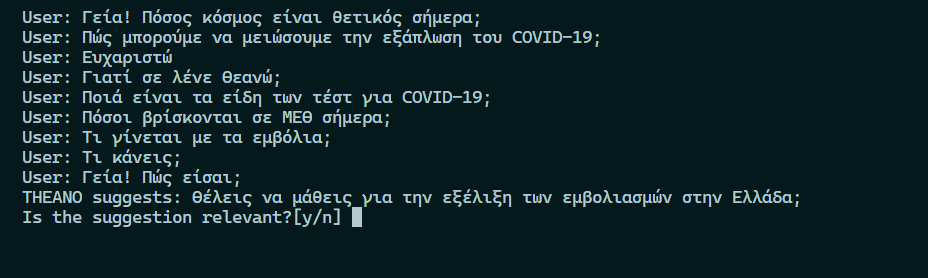
\includegraphics[width=\textwidth]{body_matter/our_work/images/rlhf_sample.png}
    \caption{Δείγμα διαλόγου ΕΜ με ανθρώπινη ανατροφοδότηση}
    \label{fig:rl_hf}
\end{figure}

% TODO add results

\section{Ενσωμάτωση με το \en{Rasa}}

Εφόσον δημιουργήσαμε μια πολιτική, θα πρέπει να την ενσωματώσουμε στο \en{Rasa} για να μπορέσουμε να την εκπαιδεύσουμε περαιτέρω σύγχρονα.

\subsection{Αρχική προσέγγιση}

Η αρχική προσέγγιση που δοκιμάσαμε ήταν η προσθήκη της πολιτικής/του μοντέλου μέσα στην προϋπαρχουσα συνάρτηση που υπήρχε στον \en{action server}. Για να το κάνουμε αυτό, χρειάζεται αρχικά να εξάγουμε πληροφορίες από την καταγραφή της κατάστασης του \en{Rasa}. Έτσι εξάγουμε τις τιμές των μακροχρόνιων πληροφοριών, τις προηγούμενες προθέσεις του χρήστη και δημιουργούμε τις εναπομείνασες προθέσεις. Αν δεν έχει μείνει καμία πρόθεση, το οποίο σημαίνει ότι όλα τα θέματα που είναι διαθέσιμα από την Θεανώ έχουν συζητηθεί, τότε χρησιμοποιούμε την γενική πρόθεση \en{\texttt{no\_action}} που αντιστοιχεί στην ερώτηση "Θα ήθελες να μάθεις κάτι άλλο?".

Αν υπάρχουν επιπλέον προτάσεις, τότε καλείται η συνάρτηση \en{\texttt{smart\_suggest}}, η οποία επικαλείται η πολιτική για να κάνει πρόταση. Για χρησιμοποιηθούν τα δεδομένα ως είσοδος στην πολιτική του \en{Vowpal Wabbit}, χρειάζεται να μετατραπούν στην μορφή εισόδου που αποδέχεται αυτό.

Η έξοδος της πολιτικής είναι μια συνάρτηση πυκνότητας πιθανότητας, δηλαδή μια λίστα από πιθανότητες, η καθεμία από τις οποίες αντιστοιχεί σε μια δράση. Δηλαδή η πιθανότητα στην αντίστοιχη θέση στην λίστα αντιστοιχεί στην πιθανότητα επιλογής της συγκεκριμένης δράσης. Έτσι για να καταλήξουμε σε κάποια απόφαση/δράση θα πρέπει να δειγματοληπτήσουμε αυτή την λίστα.

Για παράδειγμα, δοθεισας μιας λίστας $[0.7, 0.1, 0.1, 0.1]$, θα επιλέγαμε το πρώτο αντικείμενο με πιθανότητα $70\%$.

Με αυτή την δειγματοληψία, καταλήγουμε τελικά σε μια δράση/σύσταση από την πολιτική μας για το τι να προτείνει η Θεανώ ως επόμενο θέμα συζήτησης.

Όσον αφορά την σύγχρονη εκπαίδευση με βάση την αντίδραση του χρήστη στην πρόταση της Θεανώς, η προσέγγιση μας ήταν την επόμενη φορά που καλείται η λειτουργικότητα της πρότασης, να γίνεται πρώτα μια αναζήτηση του ιστορικού για τον εντοπισμό της αντίδρασης του χρήστη. Αυτή η προσέγγιση αποδείχτηκε προβληματική, καθώς η αναζήτηση στην πορεία του διαλόγου είναι περίπλοκη, μιας και μπορούν να υπάρχουν πολλά βήματα διαλόγου μεταξύ της πρώτης κλήσης της σύστασης και της δεύτερης.

Μια περιγραφής της επικοινωνίας μεταξύ \en{Rasa}, \en{Rasa Action server} και χρήστη φαίνεται στο Σχήμα~\ref{fig:rasa_sequence}. Αυτό που παραλείπεται είναι η διαδικασία μέσα στον \en{Rasa Action server}, η οποία περιγράφηκε παραπάνω.

\begin{figure}
    \centering
    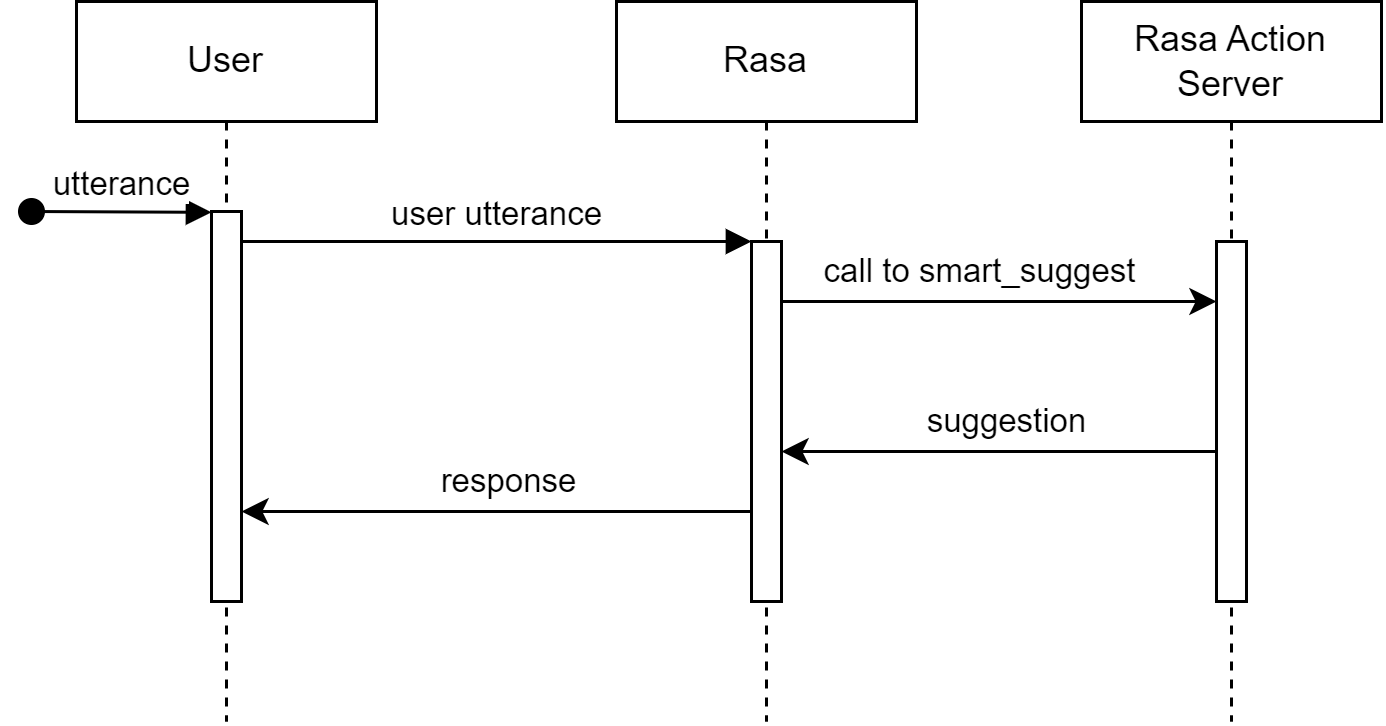
\includegraphics[width=0.7\textwidth]{body_matter/our_work/images/Rasa_ActionServer.png}
    \caption{Ακολουθιακό διάγραμμα επικοινωνίας μεταξύ \en{Rasa} και χρήστη}
    \label{fig:rasa_sequence}
\end{figure}

\subsubsection{Εξωτερική υπηρεσία}

Για να μπορέσουμε να έχουμε καλύτερη γνώση της απάντησης του χρήστη, και άρα να μπορέσουμε να υπολογίσουμε την ανταμοιβή χρειαζόμαστε πιο άμεση πρόσβαση στην πληροφορία της κατάστασης του διαλόγου του \en{Rasa}.

Για το σκοπό αυτό, καταλήξαμε ότι ο πιο άμεσος τρόπο να πάρουμε πληροφορίες για τον διάλογο ήταν με την ενσωμάτωση ενός προσαρμοσμένου καναλιού (\en{custom channel}), μιας επέκτασης που προσφέρει το \en{Rasa}. Ο σκοπός των προσαρμοσμένων καναλιών είναι η εύκολη επέκταση του \en{Rasa} σε περισσότερες πλατφόρμες φωνής και κειμένου. Μέσα σε αυτό το κανάλι όμως, μπορούμε να προσθέσουμε και επιπλέον λογική, η οποία θα μας επιτρέψει να καλούμε μια εξωτερική υπηρεσία, ένα τελικό σημείο μιας διεπαφή προγραμματισμού εφαρμογών  (\en{API endpoint}), στην οποία θα στέλνεται η κατάσταση του διαλόγου. Ο κώδικας του προσαρμοσμένου καναλιού καλείται κάθε φορά που ο χρήστης στέλνει κάτι προς το \en{Rasa}.

Αυτή η αλλαγή απαιτεί κάποιες σημαντικές αλλαγές στην αρχιτεκτονική του συνολικού συστήματος. Συγκεκριμένα, πέρα από το προσαρμοσμένο κανάλι, θα πρέπει να δημιουργήσουμε την εξωτερική υπηρεσία, η οποία θα είναι πλεον υπεύθυνη για την διαχείριση της πολιτικής, τόσο την πρόβλεψη όσο και την σύγχρονη εκπαίδευση. Επιπλέον, o \en{action server} θα πρέπει να καλεί την εξωτερική αυτή υπηρεσια για να κάνει την πρόβλεψη.

Η υπηρεσία αυτή δημιουργήθηκε έχοντας υπόψιν την έννοια των μίκρο-υπηρεσιών (\en{micro-services}), υπηρεσιών δηλαδή που υπηρετούν ένα και μοναδικό σκοπό. Στην περίπτωση μας αυτός ο σκοπός είναι η περίκλειση της πολιτικής. Έτσι αυτή η υπηρεσία έχει δύο άκρα που επικοινωνεί με το εξωτερικό περιβάλλον της. Το πρώτο είναι το \en{\texttt{/suggest}}, το οποίο λαμβάνει δεδομένα για την κατάσταση του διαλόγου του χρήστη και με βάση αυτά παράγει και επιστρέφει μια σύσταση για την συνέχεια της συζήτησης. Το δεύτερο είναι το \en{\texttt{/intent}}, το οποίο καλείται όταν ο χρήστης στέλνει κάποιο μήνυμα στην Θεανώ. Η λειτουργικότητα του είναι να ελέγχει αν έχει γίνει σύσταση προς τον χρήστη, και αν έχει γίνει να αξιολογεί την ανταπόκριση του χρήστη και με βάση αυτή να μοντελοποιεί την ανταμοιβή. Τα δεδομένα σχετικά με την κατάσταση κάθε διαλόγου αποθηκεύονται σε μια προσωρινή βάση δεδομένων και κάθε μια ώρα καθαρίζονται. Με αυτό τον τρόπο μπορούμε να ελέγξουμε και αν ο χρήστης έφυγε από την συνομιλία μετά απο μια σύσταση και να εκπαιδεύσουμε την πολιτική με βάση αυτό.

Για να δημιουργήσει το \en{Rasa} την κατάσταση του διαλόγου, θα πρέπει πρώτα το αίτημα του χρήστη να περάσει μέσα από το κανάλι και το ίδιο το \en{Rasa} για να δημιουργηθεί η κατάσταση αυτή πρώτα. Έτσι το κανάλι καλεί την υπηρεσία μας και της μεταφέρει την πρόθεση του μόνο αφού το αίτημα του χρήστη έχει περάσει μέσα από \en{Rasa}. Όλα τα παραπάνω, γίνονται αρκετά εμφανή στο Σχήμα~\ref{fig:rasa_sequence_smart_suggest_ms}.

\begin{figure}
    \centering
    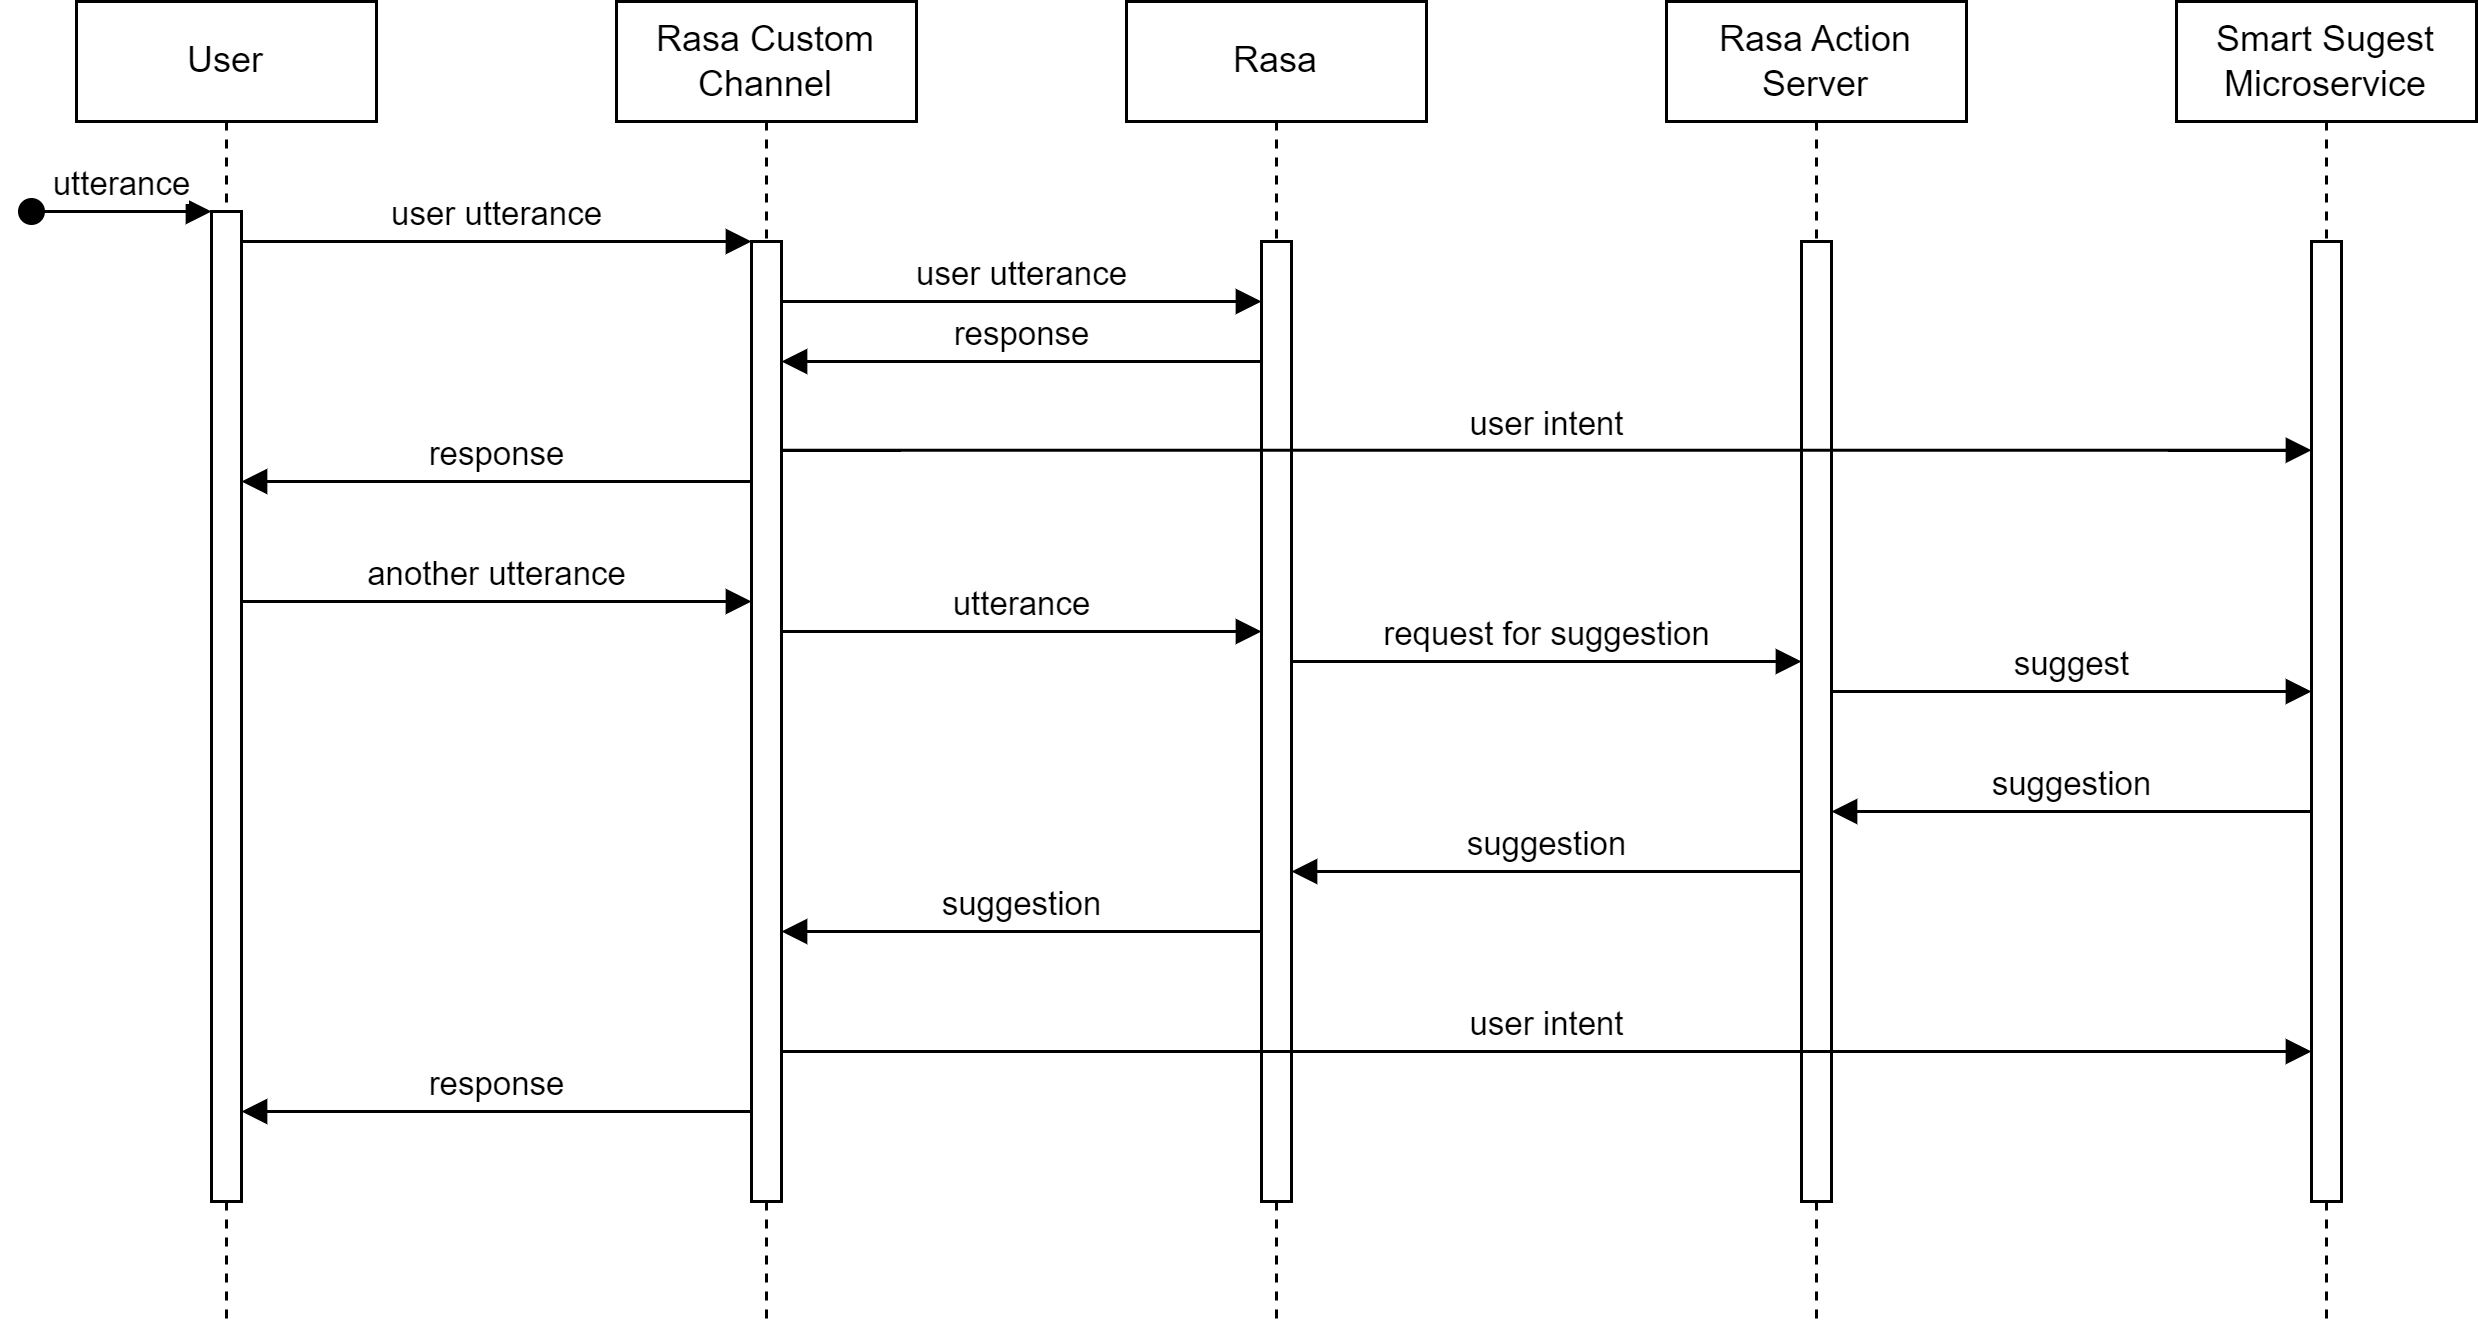
\includegraphics[width=0.7\textwidth]{body_matter/our_work/images/Rasa_smart_service.png}
    \caption{Ακολουθιακό διάγραμμα επικοινωνίας μεταξύ \en{Rasa} και χρήστη, όταν χρησιμοποιούμε την εξωτερική υπηρεσία.}
    \label{fig:rasa_sequence_smart_suggest_ms}
\end{figure}


